\chapter{RoboRef}
\label{sec:methodology}

% Citation keys used here (verify against Zotero): robometer, roboreward,
%   yu_meta-world_2019, mclean_meta-world_2025, lin_failsafe_2025.
% ManiSkill is named but not cited; add a key if we want one.

This chapter describes RoboRef. We keep Robometer's backbone and its per-frame design, analyzed in Chapter~\ref{sec:robometer}, and we change three things: the data the model learns from, the way it reads a demonstration alongside the trajectory it has to score, and the loss it minimizes. We describe the dataset first, because both the changes to the model and the experiments depend on it. We then turn to the in-context demonstrations, the asymmetric objective, and how we train the model variants we compare. The protocol we use to evaluate the resulting models, both offline and as a reward for downstream reinforcement learning, is presented alongside the results in Chapter~\ref{sec:results}.

\section{A failure-annotated dataset}
\label{sec:method-dataset}

Chapter~\ref{sec:robometer} established the gap we start from. Robometer trains its two deployment heads, progress and success, only on successful trajectories, where assuming that an expert advances steadily toward the goal hands each frame a target for free. Failed attempts reach the model only through the preference head, as the lower-ranked side of a comparison, so neither deployment head ever sees failure as a direct target. The two heads are not equally hard to fix. The success head needs only a per-frame binary flag, and for a failed attempt that flag is simply zero at every frame, since the task is never completed. The progress head is the difficult one. It needs a dense progress value at every frame, and for a failure that value does not follow from the frame index, because a failed attempt does not advance steadily. What is missing is therefore a corpus whose failures carry dense per-frame progress, and to our knowledge no such corpus exists. We build one by re-curating and expanding RBM-1M, the corpus behind Robometer.

\subsection{Re-curating RBM-1M}

We make five changes to the corpus.

\begin{itemize}
    \item We hold the humanoid and human-only data out of the main training corpus. RBM-1M draws a large share of its size from humanoid robots and from human videos, which broaden its visual coverage but sit far from the single-arm manipulation our downstream tasks involve. Keeping them out of the shared corpus sharpens it around the embodiments we focus on. However, we do not discard them completely. We keep a smaller sample and use it in our model ablations (Section~\ref{sec:method-training}), where their extra visual coverage feeds the pretraining of one variant.
    \item We replace Robometer's FailSafe split with our own. FailSafe \citep{lin_failsafe_2025} is a simulated set of contact-rich cube tasks, lifting, pushing, and stacking a block on a tabletop. We discard their version and generate a fresh set of FailSafe failures in simulation, labeled densely (Section~\ref{sec:method-sim-failures}).
    \item RoboReward \citep{roboreward} released a dataset alongside its reward model, and RBM-1M incorporates a portion of it. We replace this RoboReward split with our own. It supplies two kinds of failure data, semantically wrong executions produced by counterfactual instruction relabeling (e.g. \textit{pick up the kettle} becomes \textit{pick up the spoon}), and genuine partial executions that stop before the task is finished. We discard the whole original split and draw a smaller sample of the partial executions alone, labeled by their own clip scores. Section~\ref{sec:method-roboreward} explains the replacement and the labeling.
    \item We add DROID \citep{khazatsky_droid_2024} failures. DROID is a large real-world dataset of a robot arm performing everyday tabletop manipulation across many scenes and tasks. Robometer uses DROID for successful demonstrations only; we add failed attempts, and alongside them a small set of successful DROID clips from the same tasks and camera setups. Keeping matching successes is deliberate. Our in-context training (Section~\ref{sec:method-icl}) pairs every trajectory with a successful demonstration of the same task, so each pool of added failures needs same-task successes to draw those demonstrations from. We follow the same rule for the other failure sources we add.
    \item We add MetaWorld \citep{yu_meta-world_2019, mclean_meta-world_2025} data, mostly failures, generated from scratch in simulation (Section~\ref{sec:method-sim-failures}). MetaWorld is a simulated benchmark of a single robot arm across 46 tabletop manipulation tasks, from reaching and pushing to pick-and-place and operating buttons and drawers. RBM-1M already carried a small MetaWorld set, the 100 demonstrations from ReWiND \citep{zhang_rewind_2025}, which we drop in favor of our own.
\end{itemize}

Table~\ref{tab:roboref-dataset} reports the resulting mix. The single-arm corpus that every model shares holds $648{,}714$ rows, of which $116{,}786$ are failures and $531{,}928$ are successes. The bulk of the successes are the standard-arm expert demonstrations we retain from RBM-1M; the failures come from the four sources we add or replace plus the Robometer failures we keep and label for the first time. The humanoid and human-only pool sits apart from this. It adds a further $214{,}427$ successful trajectories, used only in the Qwen3.5 pretraining phase and shown as a separate block at the foot of the table, which brings the full corpus to $863{,}141$ rows. Appendix~\ref{apx:rbm1m} gives the full composition of RBM-1M itself, Appendix~\ref{apx:roboref-data} expands Table~\ref{tab:roboref-dataset} to one row per upstream source together with the labeling, pairing, and sampling details, and Appendix~\ref{apx:gallery} lists the simulated task families and their failure modes in full.

\begin{table*}[t]
\centering
\footnotesize
\caption[Composition of the RoboRef dataset]{Composition of the RoboRef dataset. A row is one scored video clip, that is, one episode rendered from one camera view. \emph{Provenance} states whether a source is retained from RBM-1M, replaced with our own version, or newly added. \emph{Failure labels} names where the dense per-frame failure labels come from; successful trajectories everywhere use Robometer's $t/T$ heuristic. The block at the foot holds the humanoid and human-only data, which every model leaves out of shared training and only the Qwen3.5 model sees, in its first phase alone. Counts are not directly comparable to Robometer's Table~IX, which reports unique video-language annotations expanded across views.}
\label{tab:roboref-dataset}
\begin{tabular}{@{}p{4.6cm}p{1.8cm}p{2.4cm}rrr@{}}
\toprule
Source & Provenance & Failure labels & Failures & Successes & Total \\
\midrule
Robometer expert demonstrations & retained & --- & 0 & 490{,}798 & 490{,}798 \\
Robometer mixed-expertise archives & retained & VLM+LLM & 68{,}923 & 26{,}029 & 94{,}952 \\
\addlinespace
MetaWorld (ours) & added & simulator physics & 24{,}402 & 1{,}850 & 26{,}252 \\
FailSafe (ours) & replaced & simulator physics & 2{,}098 & 75 & 2{,}173 \\
DROID (ours) & added & VLM+LLM & 5{,}503 & 5{,}863 & 11{,}366 \\
RoboReward (ours) & replaced & ramp to clip score & 15{,}860 & 7{,}313 & 23{,}173 \\
\midrule
Standard-arm total & & & 116{,}786 & 531{,}928 & 648{,}714 \\
\midrule
\multicolumn{6}{@{}l}{\emph{Held out of shared training; used only for the Qwen3.5 first phase}}\\
Humanoid & retained & --- & 0 & 112{,}629 & 112{,}629 \\
Human-only & retained & --- & 0 & 101{,}798 & 101{,}798 \\
\midrule
Total with phase-1 data & & & 116{,}786 & 746{,}355 & 863{,}141 \\
\bottomrule
\end{tabular}
\end{table*}

\subsection{Labeling failures densely}

A successful demonstration is almost free to label. As we explained in previous chapters, if a clip has $T$ frames and the expert reaches the goal at the end, we set the progress at frame $t$ to $t/T$, a value that climbs evenly from zero at the first frame to one at the last. A failure has no such reference. It may stall, drift away from the task, or briefly approach success and then fall apart, so its progress does not climb steadily and cannot be read off the frame index. Which route we take to label a failure depends on its dataset family. 

For the failures we generate ourselves in simulation, MetaWorld and FailSafe, we have the simulator's true state and read progress straight from it (Section~\ref{sec:method-sim-failures}). For the rest of the failures where we only possess a recorded video, we infer progress from the frames with a two-stage model pipeline (Section~\ref{sec:method-real-failures}). This video-only group is larger than it first appears. It covers the real-world failure clips already in RBM-1M and the DROID failures we add. It also contains some simulated data already in RBM-1M from other dataset families, such as RACER \citep{dai_racer_2025} evaluated in RLBench \citep{james_rlbench_2020}, whose videos we keep but whose simulator we never run due to time constraints. The RoboReward partial executions are a third, unique, case (Section~\ref{sec:method-roboreward}). Since they are shortened clips of actual demonstrations, they are monotone by construction. Thus, they are labeled by the simple ramp that successes used, described above. So, they need neither of the two routes.

Whatever the route, every failure label lands on one common scale. Each failure frame first gets a rubric score $s \in \{1,2,3,4,5\}$, which we map to a normalized progress value $p = (s-1)/4$, so the five levels become $\{0, 0.25, 0.5, 0.75, 1.0\}$. A genuine failure never completes the task, so its scores stay in $\{1,2,3,4\}$ and its progress never reaches $1.0$.

However, this format is different from the one that successes use, as these per-frame scores would give a failure a stair-step target, flat within a level and jumping at each change of level, whereas a success target is the smooth $t/T$ ramp. We do not want the model to tell failures from successes by the shape of the target alone, a staircase against a ramp, so we smooth the failure target. When a training sample is built, we interpolate each failure's progress linearly between the frames where its level changes, which turns the staircase into a ramp that still passes through the rubric values. Failures and successes then share one continuous target on $[0,1]$, the scale the progress head predicts over, and the successes keep their $t/T$ labels untouched. 

One could in principle relabel the successes with the same two-stage pipeline we use for the video failures (Section~\ref{sec:method-real-failures}) to remove this asymmetry, but its language-model stage is expensive and the success corpus is far too large for that to be practical, so the successes stay on the cheap $t/T$ heuristic. Furthermore, someone could argue that the pure monotonicity of the success data could discriminate between success and failure data. Thus, in preliminary experiments described in Chapter~\ref{sec:results} we also tried to add noise to success labels and break their pattern; however, it proved suboptimal in our experiments.

This normalized progress value $p$ is then encoded for the progress head exactly as described in Chapter~\ref{sec:robometer}. The value is projected into a discrete target distribution over $N=10$ bins, and the progress head is trained using a cross-entropy loss between this target and its own prediction. Simultaneously, the success head is trained on a binary completion flag, which remains strictly zero at every frame of a failed trajectory.

\subsection{Simulated failures}
\begin{figure*}[t]
\centering
% Frames are simulator renders (raster); the label curve below is PGFPlots (code).
% FailSafe stack carry_drop inst0002, eight of sixteen keyframes; labels 1 1 2 3 3 3 1 1.
\begin{subfigure}{\textwidth}
\centering
\begin{tikzpicture}
% frames live inside the axis (axis cs) so they sit exactly above the curve points
\begin{axis}[scale only axis, width=0.944\textwidth, height=2.4cm,
  xmin=0.5, xmax=8.5, xtick=\empty, ymin=0.7, ymax=4.3, ytick={1,2,3,4},
  ylabel={Score}, axis lines=left, ymajorgrids, grid style={gray!18},
  tick label style={font=\scriptsize}, label style={font=\footnotesize},
  enlarge x limits=false, clip=false]
\addplot[thick, mark=*, mark size=1.5pt, color=blue!65!black]
  coordinates {(1,1)(2,1)(3,2)(4,3)(5,3)(6,3)(7,1)(8,1)};
\node[anchor=south, inner sep=0, yshift=2pt] at (axis cs:1,4.3) {
\includegraphics[width=0.118\textwidth]{media/sim/failsafe/f0.jpg}};
\node[anchor=south, inner sep=0, yshift=2pt] at (axis cs:2,4.3) {
\includegraphics[width=0.118\textwidth]{media/sim/failsafe/f1.jpg}};
\node[anchor=south, inner sep=0, yshift=2pt] at (axis cs:3,4.3) {
\includegraphics[width=0.118\textwidth]{media/sim/failsafe/f2.jpg}};
\node[anchor=south, inner sep=0, yshift=2pt] at (axis cs:4,4.3) {
\includegraphics[width=0.118\textwidth]{media/sim/failsafe/f3.jpg}};
\node[anchor=south, inner sep=0, yshift=2pt] at (axis cs:5,4.3) {
\includegraphics[width=0.118\textwidth]{media/sim/failsafe/f4.jpg}};
\node[anchor=south, inner sep=0, yshift=2pt] at (axis cs:6,4.3) {
\includegraphics[width=0.118\textwidth]{media/sim/failsafe/f5.jpg}};
\node[anchor=south, inner sep=0, yshift=2pt] at (axis cs:7,4.3) {
\includegraphics[width=0.118\textwidth]{media/sim/failsafe/f6.jpg}};
\node[anchor=south, inner sep=0, yshift=2pt] at (axis cs:8,4.3) {
\includegraphics[width=0.118\textwidth]{media/sim/failsafe/f7.jpg}};
\end{axis}
\end{tikzpicture}
\caption[FailSafe stack, dropped]{FailSafe stack: a cube grasped and carried, then dropped to the table. The score climbs to $3$ and falls back to $1$.}
\end{subfigure}

\vspace{5pt}

% MetaWorld pick-place late_drop inst0005, eight of sixteen keyframes; labels 1 1 2 3 4 3 3 3.
\begin{subfigure}{\textwidth}
\centering
\begin{tikzpicture}
\begin{axis}[scale only axis, width=0.944\textwidth, height=2.4cm,
  xmin=0.5, xmax=8.5, xtick=\empty, ymin=0.7, ymax=4.3, ytick={1,2,3,4},
  ylabel={Score}, axis lines=left, ymajorgrids, grid style={gray!18},
  tick label style={font=\scriptsize}, label style={font=\footnotesize},
  enlarge x limits=false, clip=false]
\addplot[thick, mark=*, mark size=1.5pt, color=blue!65!black]
  coordinates {(1,1)(2,1)(3,2)(4,3)(5,4)(6,3)(7,3)(8,3)};
\node[anchor=south, inner sep=0, yshift=2pt] at (axis cs:1,4.3) {
\includegraphics[width=0.118\textwidth]{media/sim/metaworld/f0.jpg}};
\node[anchor=south, inner sep=0, yshift=2pt] at (axis cs:2,4.3) {
\includegraphics[width=0.118\textwidth]{media/sim/metaworld/f1.jpg}};
\node[anchor=south, inner sep=0, yshift=2pt] at (axis cs:3,4.3) {
\includegraphics[width=0.118\textwidth]{media/sim/metaworld/f2.jpg}};
\node[anchor=south, inner sep=0, yshift=2pt] at (axis cs:4,4.3) {
\includegraphics[width=0.118\textwidth]{media/sim/metaworld/f3.jpg}};
\node[anchor=south, inner sep=0, yshift=2pt] at (axis cs:5,4.3) {
\includegraphics[width=0.118\textwidth]{media/sim/metaworld/f4.jpg}};
\node[anchor=south, inner sep=0, yshift=2pt] at (axis cs:6,4.3) {
\includegraphics[width=0.118\textwidth]{media/sim/metaworld/f5.jpg}};
\node[anchor=south, inner sep=0, yshift=2pt] at (axis cs:7,4.3) {
\includegraphics[width=0.118\textwidth]{media/sim/metaworld/f6.jpg}};
\node[anchor=south, inner sep=0, yshift=2pt] at (axis cs:8,4.3) {
\includegraphics[width=0.118\textwidth]{media/sim/metaworld/f7.jpg}};
\end{axis}
\end{tikzpicture}
\caption[MetaWorld pick-place, dropped]{MetaWorld \texttt{pick-place}: the puck lifted toward the goal, then dropped. The score reaches $4$ and falls back to $3$.}
\end{subfigure}

\caption[Dense non-monotonic failure labels from simulation]{Dense, non-monotonic failure labels from simulation. Each strip shows eight keyframes of a failed attempt, and the curve beneath plots the per-frame progress score read directly from the simulator state. In both cases the score rises as the arm makes progress and then regresses when the object is dropped. These plotted scores are the ground-truth training targets.}
\label{fig:sim-failures}
\end{figure*}

\label{sec:method-sim-failures}

In simulation we do not collect failures and then label them. We choose a target rubric score and attempt to generate a failure whose progress lands on it. For a task and a target score, the pipeline runs a scripted expert until a pre-defined signal, a progress measure such as the gripper-to-object distance or the grasp flag, crosses a task-specific injection point. Once that happens, it switches to a noise mode that induces a particular kind of failure and runs on for only a short, fixed number of steps before we end the episode. The MetaWorld pick-place episode in Figure~\ref{fig:sim-failures} is one such near-success failure. The scripted expert lifts the puck and carries it almost to the goal, and only there does the noise controller force the gripper open, so the puck drops and the attempt fails just short. Keeping this post-injection phase short is deliberate. If the robot flailed under noise for a long time, the sixteen frames we later subsample would be dominated by that phase and leave too few for the clean run-up before the failure. The injection point fixes how far the attempt gets before it breaks. For a target of one the noise starts at once, for two once the arm has reached the object, for three once the object is grasped and moved, and for four only deep into the task. We keep an episode only if the simulator's state-based detector confirms it ended at the intended score, then subsample it uniformly to sixteen frames.

The noise modes are specific to each simulator. MetaWorld uses nine. They are \emph{random} (fully random actions), \emph{wrong-direction} (a strong bias away from the goal), \emph{freeze} (the arm holding position with a fraction of the expert's force), \emph{drop} (the gripper forced open mid-transport), \emph{late-drop} (the gripper forced open just short of the goal, Figure~\ref{fig:sim-failures} bottom), \emph{misplace} (the expert action plus a small offset near the goal), \emph{lift-away} (the arm lifting off and losing contact), \emph{push-sideways} (the arm pushing perpendicular to the goal), and \emph{partial-actuation} (the expert driving a mechanism or button most of the way and then stalling short of completion). Which modes apply depends on the task family and the target score. A grasping task reaches its near-complete failures through \emph{drop} and \emph{late-drop}, a pushing task through \emph{lift-away} and \emph{push-sideways}, and a mechanism or button through \emph{partial-actuation}, while \emph{random}, \emph{wrong-direction}, and \emph{freeze} cover the low scores everywhere. Appendix~\ref{apx:gallery} gives the full task-and-mode breakdown. FailSafe builds its three cube tasks from the analogous behaviors: moving away from the cube, freezing before contact, approaching and then retreating, grasping and then freezing, carrying without releasing, dropping mid-carry (Figure~\ref{fig:sim-failures} top), and, near the goal, releasing or nudging the cube just short of success. A handful of runs complete the task for an instant and are then disturbed, so the cube is knocked back out of place.

Because the simulator exposes the true state at every step, the per-frame progress comes straight from physics, with no model in the loop. This gives us the property we care about most. The label tracks the behavior, and it falls when the behavior regresses. When the arm drops a grasped object the progress steps back down, and when a briefly completed task is disturbed it falls from the top of the scale. A monotone $t/T$ label cannot represent this backward motion, and it is exactly what we want the progress head to learn to read.

We generate two such sets. MetaWorld \citep{yu_meta-world_2019, mclean_meta-world_2025} gives a simulated Sawyer robot arm over 46 manipulation tasks, with failures at every pre-success score. We hold a subset of the tasks out of training and reserve them for evaluation, so no task seen at test time appears during training. FailSafe, built in the ManiSkill simulator \citep{mu_maniskill_2021, tao_maniskill3_2024}, gives the three contact-rich cube tasks above, where the hardest cases reach a near-success score before failing. Every episode is rendered from three camera viewpoints, and because the labels come from physics and not pixels they are identical across the three views.


\subsection{Real-world failures}
\begin{figure*}[t]
\centering
% Per-frame (unrolled) view. Frames are raster DROID renders; everything else is TikZ.
% Frames, descriptions, and scores are real outputs. Prompts are in the appendix.
\resizebox{\textwidth}{!}{%
\begin{tikzpicture}[
  font=\footnotesize, >={Latex[length=2.2mm]},
  frame/.style={draw=gray!45, inner sep=1pt, rounded corners=1pt},
  desc/.style ={draw=teal!55!black, fill=teal!8, rounded corners=3pt, align=left,
                inner sep=4pt, text width=5.0cm, font=\scriptsize},
  grade/.style={draw=orange!80!black, fill=orange!16, rounded corners=3pt, align=center,
                inner sep=4pt, text width=1.7cm, font=\footnotesize},
  tlab/.style ={font=\scriptsize\itshape, text=gray!45!black},
  outtag/.style={font=\scriptsize\itshape},
  ell/.style={font=\large\bfseries, text=gray!55!black},
]
% task header
\node[anchor=west, font=\footnotesize] (hdr) at (-5.6,3.9)
  {\textbf{Task:} ``Stack 3 cups.''\quad\textcolor{gray!55!black}{8 frames sampled; three shown}};
% left stage labels (horizontal), with model names and explicit outputs
\node[anchor=east, align=left, text width=2.6cm, font=\scriptsize, text=teal!40!black] (st1) at (-2.95,-0.25)
  {\textbf{Stage 1\,---\,describe}\\[1pt]{\ttfamily\scriptsize Qwen3.5-VL-35B-A3B}\\[1pt]reads each frame on its own.\\[2pt]\emph{Output: one description per frame.}};
\node[anchor=east, align=left, text width=2.6cm, font=\scriptsize, text=orange!55!black] (st2) at (-2.95,-5.05)
  {\textbf{Stage 2\,---\,grade}\\[1pt]{\ttfamily\scriptsize Qwen3-32B}\\[1pt]reads each description with all earlier ones.\\[2pt]\emph{Output: a 1--4 score per frame.}};
% frame index labels (above the frames)
\node[tlab] (tl1) at (0,2.85)    {frame 2};
\node[tlab] (tl2) at (5.9,2.85)  {frame 7};
\node[tlab] (tl3) at (11.8,2.85) {frame 8};
% frames + ellipses (8 frames sampled; three shown)
\node[frame] (f1) at (0,1.5)    {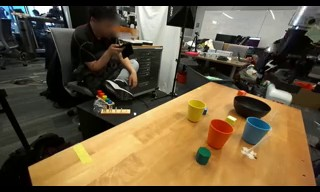
\includegraphics[width=3.8cm]{media/pipeline/cups1.jpg}};
\node[frame] (f2) at (5.9,1.5)  {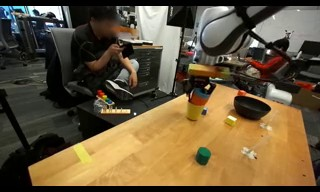
\includegraphics[width=3.8cm]{media/pipeline/cups2.jpg}};
\node[frame] (f3) at (11.8,1.5) {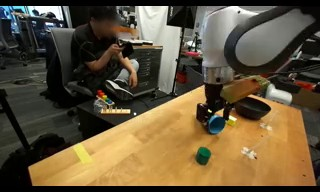
\includegraphics[width=3.8cm]{media/pipeline/cups3.jpg}};
\node[ell] at (2.95,1.5) {$\cdots$};
% descriptions (real, condensed) -- VLM output
\node[outtag, text=teal!45!black, anchor=west] at (-2.5,-0.95) {VLM output};
\node[desc] (d1) at (0,-2.0)
  {\textbf{Objects:} three cups on the table. \textbf{Gripper:} empty, above the table. \textbf{Progress:} no cups stacked yet.};
\node[desc] (d2) at (5.9,-2.0)
  {\textbf{Objects:} the cups, now stacked. \textbf{Gripper:} on the top cup. \textbf{Progress:} the stack is briefly complete.};
\node[desc] (d3) at (11.8,-2.0)
  {\textbf{Objects:} the cups, scattered on the table again. \textbf{Gripper:} empty. \textbf{Progress:} the stack has toppled; the attempt fails.};
% grade cells -- LLM output
\node[outtag, text=orange!55!black, anchor=west] at (-2.5,-4.35) {LLM output};
\node[grade] (L1) at (0,-5.05)    {{\scriptsize score}\\[1pt]{\large\textbf{1}}};
\node[grade] (L2) at (5.9,-5.05)  {{\scriptsize score}\\[1pt]{\large\textbf{4}}};
\node[grade] (L3) at (11.8,-5.05) {{\scriptsize score}\\[1pt]{\large\textbf{1}}};
% arrows
\draw[->,teal!60!black,thick] (f1) -- (d1);
\draw[->,teal!60!black,thick] (f2) -- (d2);
\draw[->,teal!60!black,thick] (f3) -- (d3);
\draw[->,thick] (d1) -- (L1);
\draw[->,thick] (d2) -- (L2);
\draw[->,thick] (d3) -- (L3);
\draw[->,orange!80!black,thick] (L1) -- node[above=1pt,font=\scriptsize,text=orange!55!black]{$+$ earlier descriptions} (L2);
\draw[->,orange!80!black,thick] (L2) -- node[above=1pt,font=\scriptsize,text=orange!55!black]{$+$ earlier descriptions} (L3);
% stage bands + outer container
\begin{scope}[on background layer]
  \node[fill=teal!5,   rounded corners=4pt, fit=(st1)(tl1)(tl3)(f1)(f3)(d1)(d3), inner sep=8pt] (b1){};
  \node[fill=orange!5, rounded corners=4pt, fit=(st2)(L1)(L3),         inner sep=8pt] (b2){};
  \node[draw=gray!45, line width=0.8pt, rounded corners=6pt, fit=(hdr)(b1)(b2), inner sep=6pt] {};
\end{scope}
\end{tikzpicture}%
}
\caption[The two-stage labeling pipeline]{Our two-stage labeling pipeline for real-world failures, unrolled over three of the eight sampled frames of one DROID episode, depicting a failed attempt to stack three cups. In the first stage a vision--language model (Qwen3.5-VL-35B-A3B) describes each frame on its own. In the second stage a language model (Qwen3-32B) grades each frame on the one-to-four failure rubric (five is not allowed to avoid hallucinations), reading the current description together with all earlier ones, which the horizontal arrows carry. The score climbs to four once the cups are stacked, then falls back when the stack topples. Stacking three cups is a multi-step task, so the language model first decomposes it into ordered sub-steps and grades against them. The detailed prompts can be found in Appendix~\ref{apx:prompts}. The frames, descriptions, and scores shown are real outputs.}
\label{fig:vlm-llm-pipeline}
\end{figure*}

\label{sec:method-real-failures}

For the failures where we have access only to the video of their trajectory, we infer the label from the frames, using two models in sequence. The first is a vision-language model, Qwen3.5-VL-35B-A3B. It looks at each frame on its own, independently of the others, and answers three fixed questions:
\begin{enumerate}
    \item which task-relevant objects are present and in what state
    \item what the gripper is doing at that moment
    \item what has been accomplished so far, measured against the goal.
\end{enumerate}
It sees one frame at a time, together with the task description, and answers in a few short sentences. Figure~\ref{fig:vlm-llm-pipeline} traces one clip through both stages, and the full prompt is in Appendix~\ref{apx:prompts}.

The second model is a language model, Qwen3-32B, which never sees the images. It reads the frame descriptions in the order they occur and assigns each one a progress score. The grading is cumulative. To score frame $t$ the model is given the descriptions of frames $1$ through $t$ along with the score it gave the previous frame, and it may lower a score only when the descriptions show that progress was genuinely undone.

The rubric it grades against has five levels, and a failure can reach only the first four. They are similar to the ones described in the simulation setup. A score of one is no meaningful progress, the arm never engaging the object the task is about. Two is contact without commitment, the object approached or touched but taken no further. Three is real partial progress, at least one sub-goal met, typically the object grasped and carried toward its target. Four is a near miss, the attempt carried almost to the end and broken only at the last moment, a grasp that slips or a placement that just fails to land. Five would mean the task is complete, which no clip in this pool is allowed to reach (without this cap, some did, due to VLM hallucinations), so the scores we collect run from one to four. Appendix~\ref{apx:prompts} gives the prompt that defines these levels in full.

However, from the above concept a specific question emerges. How would this rubric handle a task with several steps? These four levels are perfect for a one-object task such as a pick-and-place, but for stacking three cups or clearing a table they are too coarse to capture how much of the job is done. We deal with this by scanning the task descriptions across the whole corpus, separating manually the multi-step tasks from the rest, and giving them their own prompt. For such a task the language model first turns the task description into an ordered list of sub-steps, and then scores each frame by how many of those sub-steps are complete instead of against the generic four-level scale. That alternate prompt is also in Appendix~\ref{apx:prompts}.

One detail links the pipeline to the model. The VLM reads eight frames, sampled evenly across the clip, so the pipeline scores eight frames and not sixteen. This is a cost decision, as both stages run once per frame, so labeling at sixteen would have doubled the price of the whole corpus. Our model reads sixteen (Section~\ref{sec:method-arch}), so we lift the eight scores to sixteen before training. The eight labeled frames keep their scores, and each frame that falls between two of them is set to the midpoint of its two neighbors, rounded toward the earlier one. That rounding keeps the interpolation from anticipating progress. A rise of one level between two labeled frames leaves the in-between frame at the lower value, a rise of two puts it halfway, and a drop is filled the same conservative way. The simulated failures need none of this, since we label all sixteen of their frames from physics directly.

Splitting the work in two is a direct response to where these models fail, and they fail entirely on the vision side. Asked to label a whole clip at once, a VLM tends to infer instead of observe. It reads the task description, assumes the robot carried it out, and reports progress that never happened. The language model does not make this kind of mistake. It works only from text, so once the descriptions are faithful its grading is dependable, and the whole design is therefore aimed at keeping the descriptions faithful. We compared several models before settling on this pair, and report that comparison in Appendix~\ref{apx:vlm-comparison}. Two choices help most. Showing the model one frame at a time stops it from narrating a story across the clip, and instructing it in the prompt not to guess intentions or say what the robot is about to do keeps each description tied to what that frame actually shows. Some hallucination still slips through, and that is unavoidable; we accept it, on the assumption that a small fraction of noisy labels washes out over training. Finally, for the same reason we forbid the language model from ever assigning the top label \emph{five}, even though a trajectory can look momentarily complete partway through, as in Figure~\ref{fig:vlm-llm-pipeline}, before it comes apart.

One trade-off is worth recording. The single strongest guard against hallucination was to withhold the task description from the vision-language model altogether, because with the task in hand it would anchor on it and narrate the actions it expected instead of the ones in front of it. Without it, though, the descriptions occasionally drifted onto objects and events that had nothing to do with the task, and that in turn confused the grader. We keep the task description in the prompt as the smaller of the two problems, trading a little hallucination for descriptions that stay on topic. An example of the inherited hallucinations can be seen in Appendix~\ref{apx:vlm-comparison}.

Running this pipeline is far too computationally expensive to use as the reward inside a reinforcement learning loop, so it only labels our training data, while the far cheaper RoboRef model provides the reward itself.

\subsection{RoboReward partial executions}
\label{sec:method-roboreward}

Robometer inherited a portion of RoboReward's failure data, which comes in the two kinds listed above, the counterfactual relabels and the partial executions. However, we choose to drop them and re-introduce only a smaller chunk. Inside RBM-1M, there is no way to tell the failure origin of a certain datapoint, while fetching the clips directly from RoboReward's release, where the two kinds are separated, is easy. So we discard the inherited split and draw our own sample. That sample is deliberately small and holds only partial executions. Neither kind of RoboReward failure data is very realistic, and a big failure pool dominated by semantic mismatches or truncated demonstrations would drown out the failures we consider most valuable. We want to focus on the physically grounded failures from MetaWorld and FailSafe, as well as the labeled failures from the dual labeling pipeline, thus we want a smaller split from RoboReward's data.

Labeling these clips is essentially free. A partial execution is a success cut short, so its progress climbs steadily and simply stops early, and each clip already carries a single RoboReward score for how far it got, on the same one-to-five scale where five is a success. We spread that score across the clip's frames as an even ramp from the start up to the score it reached, the same construction a full success gets but ending at the clip's score and not at completion. Neither the simulator nor the labeling pipeline is needed.

These methods, the simulator, the two-model pipeline, and the RoboReward ramp give every failure in the corpus a dense per-frame progress target, which is the whole aim of the re-curation. The failures Robometer already held are also very valuable. Robometer only ever used them indirectly, as the lower-ranked side of a preference comparison, and never as a target for its progress or success head; on the dataset we have built they become direct training signal for both. With the data settled, we turn to the changes on the model itself, in-context learning and the asymmetric objective among them.


\section{Architecture}
\label{sec:method-arch}

This section sets out how RoboRef's architecture differs from Robometer's, which we described in Chapter~\ref{sec:robometer}. We keep the backbone and the per-frame design and make three changes to it. We remove one of the three prediction heads, we double the number of frames the model reads from a clip, and we let the model read a successful demonstration alongside the trajectory it has to score. We analyze them in the following sections.

\subsection{Two heads instead of three}

We remove the preference head and keep only the progress and success heads. In Robometer the preference head earned its place by pulling failure signal into training indirectly, as the lower-ranked side of a comparison, which was the only way the two task heads ever met a failed trajectory. Our dataset removes that constraint, since both task heads now train on failures directly, with dense per-frame targets. The comparison route no longer supplies anything they do not already get, so we drop it. Removing it also tightens the objective, because the two heads that remain are exactly the two the model uses at deployment. The training loss becomes
\begin{equation}
\mathcal{L} = \mathcal{L}_{\mathrm{prog}} + \mathcal{L}_{\mathrm{succ}} ,
\end{equation}
so the total objective of Equation~\ref{eq:total-loss} loses its third term, and the paired input of Equation~\ref{eq:input-pair} disappears with it. The model is now only ever asked to score a single trajectory. However, it will still have to handle more than one trajectory as an input, as we introduce in-context learning in our new formulation.

\subsection{More frames, more detailed information}

Robometer samples eight frames from a clip. We sample sixteen, evenly spaced in the same way. The reason is temporal resolution. Reading a failure well means locating the moment it turns, the instant a grasp slips or an object is dropped, and doubling the frames lets a per-frame label sit closer to that moment and exposes more of the partial progress on either side of it. The per-frame layout is otherwise unchanged, with each of the sixteen frames followed by its $\langle\mathrm{prog}\rangle$ marker. Once a demonstration is attached, described next, a single prompt carries thirty-two frames. Chapter~\ref{sec:results} reports an ablation that trains an otherwise identical eight-frame variant under the same recipe, justifying this choice. The fixed frame budget itself matters too, not just its size. Appendix~\ref{apx:length-bias} reports an earlier study of ours on RoboReward, which reads whole videos instead, and shows that its score comes to track clip length, not content. That study is what gave us the confidence that frames are the right input format, and here we take the idea one step further, doubling the budget so the model reads the same clip at a finer grain.

\subsection{In-context demonstrations}
\label{sec:method-icl}

The most visible change is that the model no longer judges a trajectory from the task description alone. We pair each trajectory it scores, the \emph{query}, with a successful demonstration of the same task, and prepend the demonstration to the query inside one prompt. Writing $d_1,\dots,d_T$ for the demonstration frames and $o_1,\dots,o_T$ for the query frames, with $T=16$, the model reads
\begin{multline}
\mathrm{Tok}(l)\;\big[\,\mathrm{Tok}(d_t)\,\langle\mathrm{prog}\rangle\,\big]_{t=1}^{T}\;\langle\mathrm{demo\_end}\rangle\\
\big[\,\mathrm{Tok}(o_t)\,\langle\mathrm{prog}\rangle\,\big]_{t=1}^{T} .
\label{eq:input-icl}
\end{multline}
The causal masking of Chapter~\ref{sec:robometer} still holds over the input of Equation~\ref{eq:input-icl}, so each query frame attends back over the whole demonstration and over the query up to that point. The demonstration is context only. We supervise the per-frame markers of the query alone, and the text prompt states plainly that the model should score the trajectory to evaluate and not the demonstration.

A demonstration helps because a task description is a thin account of success. The phrase ``stack the cups'' does not say how a finished stack looks for this gripper, in this scene, from this camera, whereas a successful clip shows it exactly. Giving the model a concrete visual target, not a sentence, sharpens its judgment of whether the query has reached that target and how far along it is.

We do not attach a demonstration to every sample. With a fixed probability of $0.5$ we include one, and otherwise present the query on its own. Training both ways, instead of always conditioning on a demonstration, matters for two reasons. The model must still return a sensible score when no demonstration is at hand at deployment, so it cannot come to rely on one being present. And conditioning on a demonstration for every sample would pull the weights away from the demonstration-free behavior the backbone already holds, a form of catastrophic forgetting we try to avoid. Flipping the coin per sample shows the model both versions of a trajectory, with a demonstration and without.

The demonstrations come from a pairing built ahead of training. We construct one file that links every query in the corpus to a successful trajectory of the same task, recording for each query the identifier of its partner success and the criterion under which the two were matched. The match runs down an ordered list of criteria, from strict to loose, and takes the first that fires. The first criterion is an exact match on the recording setup, the same lab, task, building, and camera scene, taken from the location metadata DROID stores for each clip, where a building is the physical site a given lab recorded in. The second keeps the same lab, task, and scene but allows a different building. The third, and loosest, keeps only the same lab and task. Same-task alone is thus the third criterion, reached only when no closer success exists. We never substitute a demonstration of a different task. Such a demonstration would still carry something useful, a concrete example of what a completed task looks like, but only a same-task success also shows the model the specific goal the query is judged against.

Some tasks hold more failures than same-task successes, so a single success is sometimes shared across several queries. We spread that reuse instead of letting it concentrate. At each criterion we prefer a success not yet drawn, and only once every candidate has been used do we reuse one, always taking the least-used success of the task so that no single demonstration is over-represented across training. This happens most with the generated simulation failures, which cover many distinct failure modes. For them we produce a large pool of oracle-driven successes from many randomized initial states and use those successes both as in-context demonstrations and as queries, though because the failures so outnumber them, they serve mostly as demonstrations.

A few queries have no same-task success anywhere in the corpus. These we leave unpaired, and for them the coin flip is overridden, so even when it calls for a demonstration we attach none and train the query on its own. This is the reason that, when we assembled the dataset in Section~\ref{sec:method-dataset}, every failure source we added was brought in together with a set of same-task successes. Had we added the failures alone, they would have had no demonstration to draw on. The unpaired queries are the minority, as the pairing finds a same-task success for close to nine samples in ten, so the missing demonstrations barely shift the overall balance between the two input forms.

The pairing is not limited to failures. A successful query is paired as well, with a different same-task success standing in as its demonstration, so the demonstration-conditioned behavior the model learns is the same whether the trajectory it scores succeeds or fails.

\section{An asymmetric objective}
\label{sec:method-loss}

Our fine-tuned reward models tend to over-predict success, reading completion into trajectories that never finish. For a reward that drives RL this is dangerous, because a false positive misleads the policy far more than a false negative \citep{gumbsch_demonstrations_2026}. The re-curated dataset of Section~\ref{sec:method-dataset} is one response, since a model that has only ever trained on success is expected to perform suboptimally on failures. The loss function is the other. The loss inherited from Robometer treats the two ways of being wrong as equals, so over-predicting progress costs as much as under-predicting it and a false alarm on the success head costs as much as a missed completion. For a model that will hand out reward inside a reinforcement learning loop, this approach is the wrong default, because the two errors are not equally harmful once a policy optimizes against the reward. A false positive, the reward calling a failed trajectory a success, plants a spurious goal that the policy will seek out and exploit, the failure mode known as reward hacking. A false negative, withholding reward from real progress, only slows learning and offers no shortcut. The reward model should therefore be more conservative.

We design a loss function that penalizes over-prediction more heavily than under-prediction, so the model settles below its targets, not above them. We build two such objectives and compare them. The first stays close to Robometer, keeping its progress and success heads and reweighting the losses that train them. The second is vastly different. It discards the head used by Robometer for a single ordinal one graded on the rubric levels directly. Figure~\ref{fig:asym-losses} previews the asymmetry each of the two builds in, and we describe both in the subsequent sections.

\begin{figure*}[t]
\centering
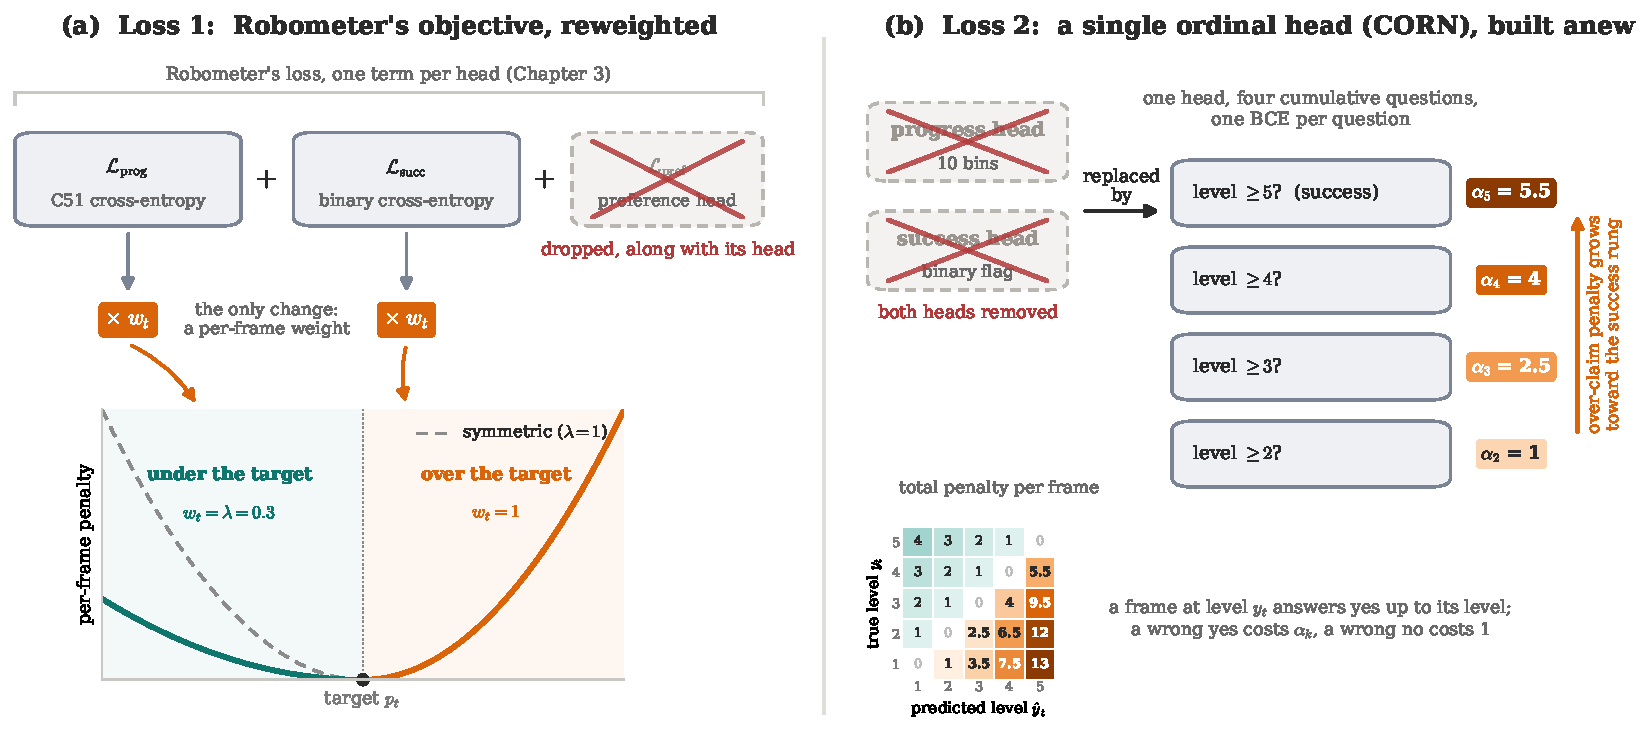
\includegraphics[width=\textwidth]{media/loss/asym_losses.pdf}
\caption[The two candidate loss objectives]{The two candidate objectives of Section~\ref{sec:method-loss}, drawn structurally. \emph{(a)} The first loss keeps Robometer's objective and its two task heads and only reweights them. The preference term is dropped together with its head, and each remaining term is multiplied by a per-frame weight $w_t$, equal to $1$ when the prediction sits above its target and $\lambda = 0.3$ when it sits below, which gives the asymmetric penalty of the lower plot, where an illustrative squared error stands in for the C51 cross-entropy. \emph{(b)} The second loss is built anew. It removes the progress and success heads entirely and replaces them with a single ordinal head that answers four cumulative questions, one binary cross-entropy per threshold, and claiming a level the frame has not reached costs $\alpha_k = 1 + c\,(k-2)$ with $c = 1.5$, heaviest at the success threshold. The matrix reads off the total penalty for every pair of true and predicted level, over-claims in orange, under-claims in teal, so the single most expensive mistake is claiming success on a frame with no progress at all.}
\label{fig:asym-losses}
\end{figure*}

\subsection{Reweighting Robometer's heads}

This objective keeps Robometer's two heads and their losses and adjusts only the weight on each frame's loss. When the model predicts too high, the frame keeps its full loss. When it predicts too low, the loss is scaled down by a factor $\lambda < 1$. An over-prediction therefore moves the weights more than an under-prediction of the same size, and the model drifts toward the low side of its targets. We use the same $\lambda$ on both heads, and $\lambda = 1$ gives back the ordinary symmetric loss. Figure~\ref{fig:asym-losses}~(a) shows the shape this induces around a target, a full-cost arm above it and a damped arm below.

On the progress head we compare, at each frame, the progress the model reports against the target. The reported value is the mean of its predicted distribution, $\bar{p}_t = \sum_{i=1}^{N} \hat{p}_{t,i}\,c_i$, with $\hat{p}_t$ the distribution over the bins with centers $c_i$ from Chapter~\ref{sec:robometer}, and $p_t$ is the target. We keep the same C51 cross-entropy as before and multiply it by a weight $w_t$ that is $1$ when $\bar{p}_t$ sits above the target and $\lambda$ when it sits at or below it,
\begin{equation}
\mathcal{L}_{\mathrm{prog}} = \frac{1}{T}\sum_{t=1}^{T} w_t\,\mathrm{CE}\!\big(\mathrm{Proj}(p_t),\, \hat{p}_t\big), \qquad
w_t = \begin{cases} 1, & \bar{p}_t > p_t,\\[2pt] \lambda, & \bar{p}_t \le p_t. \end{cases}
\label{eq:prog-asym}
\end{equation}
In Equation~\ref{eq:prog-asym}, this comparison of $\bar{p}_t$ against $p_t$ reads the current prediction only as a fixed reference, so it sets the weight for each frame without adding a gradient of its own.

On the success head over-prediction means one specific thing, calling a frame complete when it is not, so the same bias falls on the two label classes, not on a per-frame comparison. We keep the binary cross-entropy of Chapter~\ref{sec:robometer} and split it by the target. Frames that are genuinely incomplete, with $s_t = 0$, keep full weight, and frames that are complete, with $s_t = 1$, are damped by $\lambda$,
\begin{equation}
\mathcal{L}_{\mathrm{succ}} = \frac{1}{|\mathcal{N}|}\sum_{t \in \mathcal{N}} \mathrm{BCE}\!\big(0,\, \hat{s}_t\big) \;+\; \lambda\,\frac{1}{|\mathcal{P}|}\sum_{t \in \mathcal{P}} \mathrm{BCE}\!\big(1,\, \hat{s}_t\big),
\label{eq:succ-asym}
\end{equation}
In Equation~\ref{eq:succ-asym}, $\mathcal{N} = \{t : s_t = 0\}$ and $\mathcal{P} = \{t : s_t = 1\}$ are the unsuccessful and successful frames. Damping the positive class makes the model reluctant to fire a success signal, which is again the mistake we most want to suppress. A failed trajectory is unsuccessful at every frame, so all of its frames sit in the full-weight term $\mathcal{N}$, and the damped term is supplied by the successful trajectories the batch is paired with.

We use $\lambda = 0.3$ for both heads, so an under-prediction is corrected at less than a third of the strength of a matching over-prediction. Nothing else in this objective changes, and the heads, their targets, and the sum $\mathcal{L} = \mathcal{L}_{\mathrm{prog}} + \mathcal{L}_{\mathrm{succ}}$ are as in Section~\ref{sec:method-arch}, with the asymmetry living entirely in the two weights.

\subsection{Conditional Ordinal Regression for Neural Networks (CORN)}

The reweighting corrects the loss but leaves a deeper mismatch in place. Robometer's progress head predicts a distribution over ten bins and is trained by cross-entropy, which treats those bins as unordered categories. Nothing in the objective knows that the bins form a scale, that bin eight sits beside bin seven and far from bin one, so the penalty does not grow with how far a prediction lands from the target. The asymmetric weight of the previous section shares this blind spot, since it stamps a prediction as an over-prediction and applies full weight whether the model is a little too high or wildly too high. A conservative reward really wants the cost of over-prediction to scale with its size, and an ordinal formulation delivers that.

The second objective therefore replaces the ten-bin head with one that is ordinal by construction, following the rank-consistent CORN formulation \citep{shi_deep_2021}.
Instead of a distribution over bins, the head asks, for each frame, a short ladder of cumulative questions. It emits four logits $z_{t,k}$ for $k \in \{2,3,4,5\}$, and $\sigma(z_{t,k})$ is read as the probability that the frame's rubric level $y_t \in \{1,\dots,5\}$ is at least $k$. Decoding the thresholds in order recovers the level, and because they are cumulative a prediction that is off by one level fails a single threshold while one off by three fails three. Ordinal distance is now part of the loss, which is what the bin classifier lacked.

The label for a frame is that same set of yes-or-no answers. A frame at level $y_t$ answers yes to every threshold at or below its level and no to the rest, which we write as the cumulative bits $b_{t,k} = \mathbf{1}[y_t \ge k]$. For instance, a frame at level three is at least two and at least three but not four or five, so its four answers are $(1,1,0,0)$. Each threshold is trained with its own binary cross-entropy, and the asymmetry enters as a weight $\alpha_k$ on the term that fires when the true level is below the threshold, the case where the model over-claims. A single hyperparameter $c \ge 0$ fixes these weights through $\alpha_k = 1 + c\,(k-2)$, so they grow with the level. Figure~\ref{fig:asym-losses}~(b) lays out the cost structure this produces over every pair of true and predicted level. The loss is
\begin{equation}
\begin{split}
\mathcal{L}_{\mathrm{prog}} = -\frac{1}{T}\sum_{t=1}^{T} \sum_{k=2}^{5} \Big[\, & b_{t,k}\,\log\sigma(z_{t,k}) \\
&+ \alpha_k\,(1 - b_{t,k})\,\log\big(1 - \sigma(z_{t,k})\big) \Big].
\end{split}
\label{eq:corn-asym}
\end{equation}
To conclude, the loss of Equation~\ref{eq:corn-asym} asks at every frame, for each level, whether the frame has reached that level, and scores each yes-or-no answer with an ordinary binary cross-entropy, just as the success head does. The only twist is that a wrong yes, claiming a level the frame has not reached, is charged more than a wrong no, and through $\alpha_k$ that surcharge is heaviest at the top level, the one that asks whether the task is finished. Setting $c = 0$ removes the asymmetry, and we use $c = 1.5$. We also try other sets of hyperparameters analyzed in Chapter~\ref{sec:results}.

This single head also does the work of two. The top rubric level is task completion, so its threshold already answers the success question, with $\sigma(z_{t,5})$ read as the probability that the task is complete at frame $t$. Robometer's separate progress and success heads collapse into one ordinal head, the lower thresholds carrying partial progress and the top threshold carrying success. So ultimately, for this loss we use a single head.

\subsection{Two additions around the loss}
\label{sec:method-extras}

Alongside the two objectives we design two further training-time additions, both aimed at weaknesses we expect, not weaknesses we have measured, and both evaluated in the comparison of Chapter~\ref{sec:results}.

The first is a KL anchor against forgetting the failures. Two asymmetries in our corpus push the model to drift away from its failure knowledge during training. Success labels are clean $t/T$ ramps while failure labels carry labeling-pipeline noise, so the optimizer gravitates toward the clean side, and the success pool outnumbers the failure pool several times over. The anchor counteracts this and it is a standard technique against catastrophic forgetting \citep{kirkpatrick_overcoming_2016, li_learning_2016}. We keep a small first-in-first-out buffer of recently seen failures together with the progress logits the model produced for them at the time. On every success step we re-score one buffered failure with the current weights and penalize movement away from the stored prediction,
\begin{equation}
\mathcal{L} = \mathcal{L}_{\mathrm{prog}} + \mathcal{L}_{\mathrm{succ}}
+ \lambda_{\mathrm{kl}}\, \mathrm{KL}\!\big(P_{\mathrm{old}} \,\|\, P_{\mathrm{new}}\big),
\label{eq:kl-anchor}
\end{equation}
where $P_{\mathrm{old}}$ is the stored progress distribution of the buffered failure, treated as a constant, and $P_{\mathrm{new}}$ is the distribution the current model assigns to the same input, so gradient flows only through the new prediction. The KL is the standard categorical divergence over the ten progress bins, averaged over the frames that carry labels, and $\lambda_{\mathrm{kl}}$ sets how strongly the past prediction binds the present one.

The second is dropout on the task description, applied only to samples that carry an in-context demonstration. With probability one third the description is kept as written, with probability one third it is replaced by a generic phrase such as ``perform the demonstrated task'', and otherwise every word is independently dropped with a small probability. The intent is to force the model to ground its judgment in the demonstration frames, since vision-language models are known to lean on the language prior instead of the visual evidence \citep{goyal_making_2017}.

\subsection{Choosing between the losses}

The two objectives differ in one practical respect. The reweighted loss is essentially identical in form to the original loss of Robometer, performing only a reweighting, so it can resume from the pretrained weights directly, while the ordinal objective has to learn its head from scratch, since four cumulative logits do not line up with the pretrained ten-bin progress head. To decide between them we finetune Robometer with both losses as LoRA adapters \citep{hu_lora_2022} under an otherwise identical recipe and compare them. As the results in Chapter~\ref{sec:results} show, the reweighted objective is the setting we adopt for the full fine-tunes, and Appendix~\ref{apx:lambda} breaks the comparison down in full, split by split, together with the sweep behind the asymmetry strength we adopt.

\section{Training and model variants}
\label{sec:method-training}

The LoRA comparison of Section~\ref{sec:method-loss} used lightweight adapters to choose an objective cheaply. The models we actually study are full fine-tunes of the language model and the reward heads, with the vision encoder kept frozen as in Robometer's own training, sharded across H100 GPUs with Fully Sharded Data Parallel (FSDP) in the bfloat16 floating-point format, on the re-curated dataset of Section~\ref{sec:method-dataset} and with the reweighted asymmetric loss that came out ahead. On top of this shared recipe we vary two things, where training starts from and how much of our method is switched on, which gives a small grid of models.

\subsection{Two starting points}

We train from two starting points to separate what our method adds from what Robometer's own reward pretraining already provides. The first is Robometer-4B. We load the released reward model together with its pretrained progress and success heads and continue training it on our data. The second starts from the base vision-language model, Qwen3.5-4B \citep{team_qwen35-omni_2026}, with freshly initialized reward heads and no reward pretraining at all. We use Qwen3.5-4B because it is a newer and stronger base model than the Qwen3-VL that Robometer builds on, so training a reward model on top of it aims for better results while also showing how much Robometer's existing reward pretraining is worth. Because its heads start cold, the Qwen3.5 model is trained in two phases, a first pass over the fuller corpus to settle the heads and a second on the same standard-arm pool the Robometer-4B runs use. Robometer-4B, already a reward model, is fine-tuned in a single pass.

\subsection{Model ablations}

For each starting point we train three versions that switch on our contributions one at a time, so each reads against the one before it. The first is a plain fine-tune on our data that keeps Robometer's original symmetric progress and success losses and adds no demonstrations, which isolates what the re-curated failure data alone has to offer. The second replaces those losses with the asymmetric loss function that was better in Section~\ref{sec:method-loss}, the one that reweighted Robometer's original loss. The third adds in-context demonstrations on top, with the per-sample coin flip of Section~\ref{sec:method-icl}, and is the full RoboRef model. Two starting points and three versions give six trained models, which Chapter~\ref{sec:results} evaluates against each other and against the untuned Robometer baseline and other reward models.

\subsection{Optimization}

We fine-tune with AdamW \citep{loshchilov_decoupled_2019}, weight decay $0.01$, and a cosine learning-rate schedule with a $10\%$ warmup, clipping gradients to a norm of $10$ and running in bfloat16 with gradient checkpointing. Each GPU carries eight trajectories, sharded across eight H100 GPUs on two nodes. The Robometer-4B runs use a learning rate of $10^{-5}$ for $5{,}000$ steps. The Qwen3.5 runs, warming a fresh head, run at $2\times10^{-5}$ for $6{,}500$ steps in the first phase (which matches the training of Robometer-4B on top of Qwen3-VL) and $10^{-5}$ for a further $5{,}000$ steps in the second. Each trajectory is sixteen frames, and a sample carrying a demonstration adds sixteen more, as in Section~\ref{sec:method-arch}.

All runs draw from the re-curated corpus of Section~\ref{sec:method-dataset}. The Robometer-4B models train on its standard-arm portion, roughly $649$k clips with the humanoid and human data held out, while the Qwen3.5 model sees the fuller corpus in its first phase before narrowing to that same portion in its second. We reason that the humanoid robot and human dexterity data have significant information to offer to a reward model, but are unnecessary to the last finetuning stage, as the model is evaluated only in single-arm manipulator setups. Instead of keeping the corpus's natural success-heavy mix, we oversample failures during training, roughly doubling how often they are drawn, which raises their share of what the model sees from $18\%$ to about $30\%$. This way we are increasing the impact of our additional failure data, and also better balance the success/failure ratio that is heavily in favor of successes in the original mix. Two sources get their own factors on top, DROID failures because they are our scarcest real-world failures and MetaWorld successes because that source is almost all failures and its few successes would otherwise barely appear. For FailSafe we do not apply oversampling since the data come from only three tasks and that could lead to overfitting. The exact factors are listed in Appendix~\ref{apx:roboref-data}. The window subsampling and the four sample-generation strategies of Chapter~\ref{sec:robometer} are kept unchanged.
